\documentclass{article}
\usepackage[utf8]{inputenc}
\usepackage{amsmath}
\usepackage{amssymb}
%paquetes que usa el doc

\title{Trabajo de Recuperación de Examen \# 1}
\author{Luis Gerardo Morales Salazar \\Carnet: 2018-1364\\ morales181364@unis.edu.gt}
\date{14 de agosto de 2018}

% datos del encabezado o titulo del doc
\usepackage{natbib}
\usepackage{graphicx}

\begin{document}
\maketitle

\section{PREGUNTA\# 1}
El famoso matematico Euler hizo la siguiente pregunta: ¿Es possible curzar todos los puentes de Königsberg
sin pasar dos veces por el mismo puente?\\ A continuación se muestra un mapa de los puentes de Königsberg:

\begin{figure}[h!]
\centering
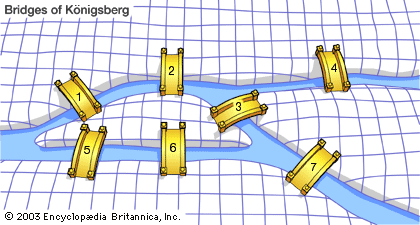
\includegraphics[scale=0.5] {bridges}
\end{figure}

\begin{enumerate}
\item Nodos del grafo: $\{1,2,3,4,5,6,7\}$

\item {El conjunto de vertices del grafo son:}
\[
        VERTICES \left\{
        \begin{array}{l l}
          <1,2>, <1,3>, <1,4>, <1,5>, <1,6> \\
          <2,4>, <2,5>, <2,6>, <2,3>, <3,4> \\
          <3,5>, <3,6>, <3,7>, <4,7>, <7,5> \\
          <7,6>, <5,6> \\
        \end{array}
        \right.
    \]
\\ \section{PREGUNTA\# 2}
Demostrar utilizando inducci\'on que la formula de Gauss para sumatorias es correcta:
\[
        \sum_{i=1}^{n}{i}=\frac{n(n+1)}{2}
\]
donde $\sum_{i=1}^{n}i=1+2+3+4+\ \ldots\ +n$.
\\\\
Para esta demostraci\'on, su caso base debe ser
$n=1$ en vez de $n=0$. Sin embargo, la demostraci\'on
del caso inductivo procede de la misma forma que
se ha estudiado en clase.
\\\\ 1. {Caso base :
\\\\ \sum_{i=1}^{n}{i}=\frac{1(1+1)}{2} 
\\\\\sum_{i=1}^{n}{i}=\frac{1(2)}{2} 
\\\\\sum_{i=1}^{n}{i}=\frac{2}{2} 
\\\\\sum_{i=1}^{n}{i}={1}}

\\\\ 2. {Caso Inductivo :
\\\\\sum_{i=1}^{n}{i}=\frac{n+1(n+1+1)}{2} 
\\\\\sum_{i=1}^{n}{i}=\frac{n+1(n+2)}{2} 
\\\\\sum_{i=1}^{n}{i}=\frac{n+1}{1} + \frac{n+2}{2} 
\\\\\sum_{i=1}^{n}{i}=\frac{n+1}{1} + (\frac{n}{2}+ \frac{2}{2}) 
\\\\\sum_{i=1}^{n}{i}=\frac{n+1}{1} + (\frac{n}{2} + 1)
\\\\\sum_{i=1}^{n}{i}=\frac{n(n+1)}{2} + \frac{n+1}{1}
\\\\\sum_{i=1}^{n}{i}=\frac{n(n+1)+2(n+1)}{2}
\\\\\sum_{i=1}^{n}{i}=\frac{(n+1)+(n+2)}{2}
\\\\\sum_{i=1}^{n}{i}=\frac{(n+1)(n+2)}{2}
\\\\\sum_{i=1}^{n}{i}=\frac{(n+1)((n+1)+1)}{1}}

\section*{PREGUNTA \#3}
Definir inductivamente la funcion $\sum(n)$ para numeros naturales unarios la cual tiene
el efecto de calcular la suma de $1$ hasta $n$. En otras palabras:
\[
        \sum(n)=1+2+3+4+\ \ldots\ +n
\]
Puede apoyarse de la suma $\oplus$ de numeros naturales unarios para su definici\'on:
\[
        a\oplus b =
                \left\{
                        \begin{array}{ll}
                                b  & \mbox{si } a = 0 \\
                                s(i\oplus b) & \mbox{si } a = s(i)
                        \end{array}
                \right.
\]
\\\\1. Definici\´on: 
\\\\\\$ \frac{s(0) (s(0) \oplus s(0))}{s(s(0))}
\\\\ \frac{s(0) (s(s(0)))}{s(s(0))}
\\\\ \frac{s(s(0))}{s(s(0))}
\\\\ s(s(0)) \ominus (\frac{s(0)}{s(0)})
\\\\ s(s(0)) \ominus s(0)) 
\\\\s(0)$


\section*{PREGUNTA \#4}
Demostrar por medio de inducci\'on la comutatividad de la suma de
numeros naturales unarios: $a\oplus b = b\oplus a$

\\ Caso base: 
\\$a = 0
\\\\0 \oplus b = b \oplus 0
\\b = b
\\\\ Caso inductivo: 
\\a = s(i)
\\\\s(i) \oplus b = b \oplus s(i)
\\s(i \oplus b) = s(b \oplus i)
\\s(i \oplus b) = s(i \oplus b)$


\section*{PREGUNTA \#5}
Dada la funci\'on $a\geq b$ para numeros naturales unarios:
\[
        a\geq b =
                \left\{
                        \begin{array}{ll}
                                s(o)  & \mbox{si } b = o \\
                                o & \mbox{si } a = o \\
                                i\geq j & \mbox{si } a = s(i)\ \&\ b = s(j)
                        \end{array}
                \right.
\]
Demostrar utilizando inducci\'on que $((n\oplus n)\geq n) = s(o)$. Puede
hacer uso de la asociatividad y comutabilidad de la suma de numeros
unarios para su demostraci\'on.
\\\\1.Caso Base: n=0
\\$((0 \oplus 0 )\geq 0)
\\(0 \oplus 0)
\\\\\\2. Demostraci\'on: n = s(0)
\\\\((s(0) \oplus s(0)) \geq s(0))
\\((s(s(0 \oplus 0))) \geq s(0))
\\((s(s(0))) \geq s(0))
\\(s(s(0)) \ominus s(0) \geq 0)
\\(s(0) \geq 0)
\\(((n \oplus n) \geq n) = s(0)) = s(0)$

% documento creado en sharelatex.com ;) 

\end{enumerate}
\end{document}